At tree level, there are three contributions to the $W^+W^+$ production in association with two jets: the pure EW component $\mathcal{O}(\alpha^6)$, the interference $\mathcal{O}(\alphas\alpha^5)$ and the QCD background $\mathcal{O}(\alphas^2\alpha^4)$.\\
The three contributions to the jet--jet invariant mass $M_{jj}$ and positive rapidity difference $|\Delta y_{jj}|$ distributions are shown in Fig.~\ref{fig:mjjdyjj_1d}, together with their sum.
\begin{figure*}[hbt]
\centering
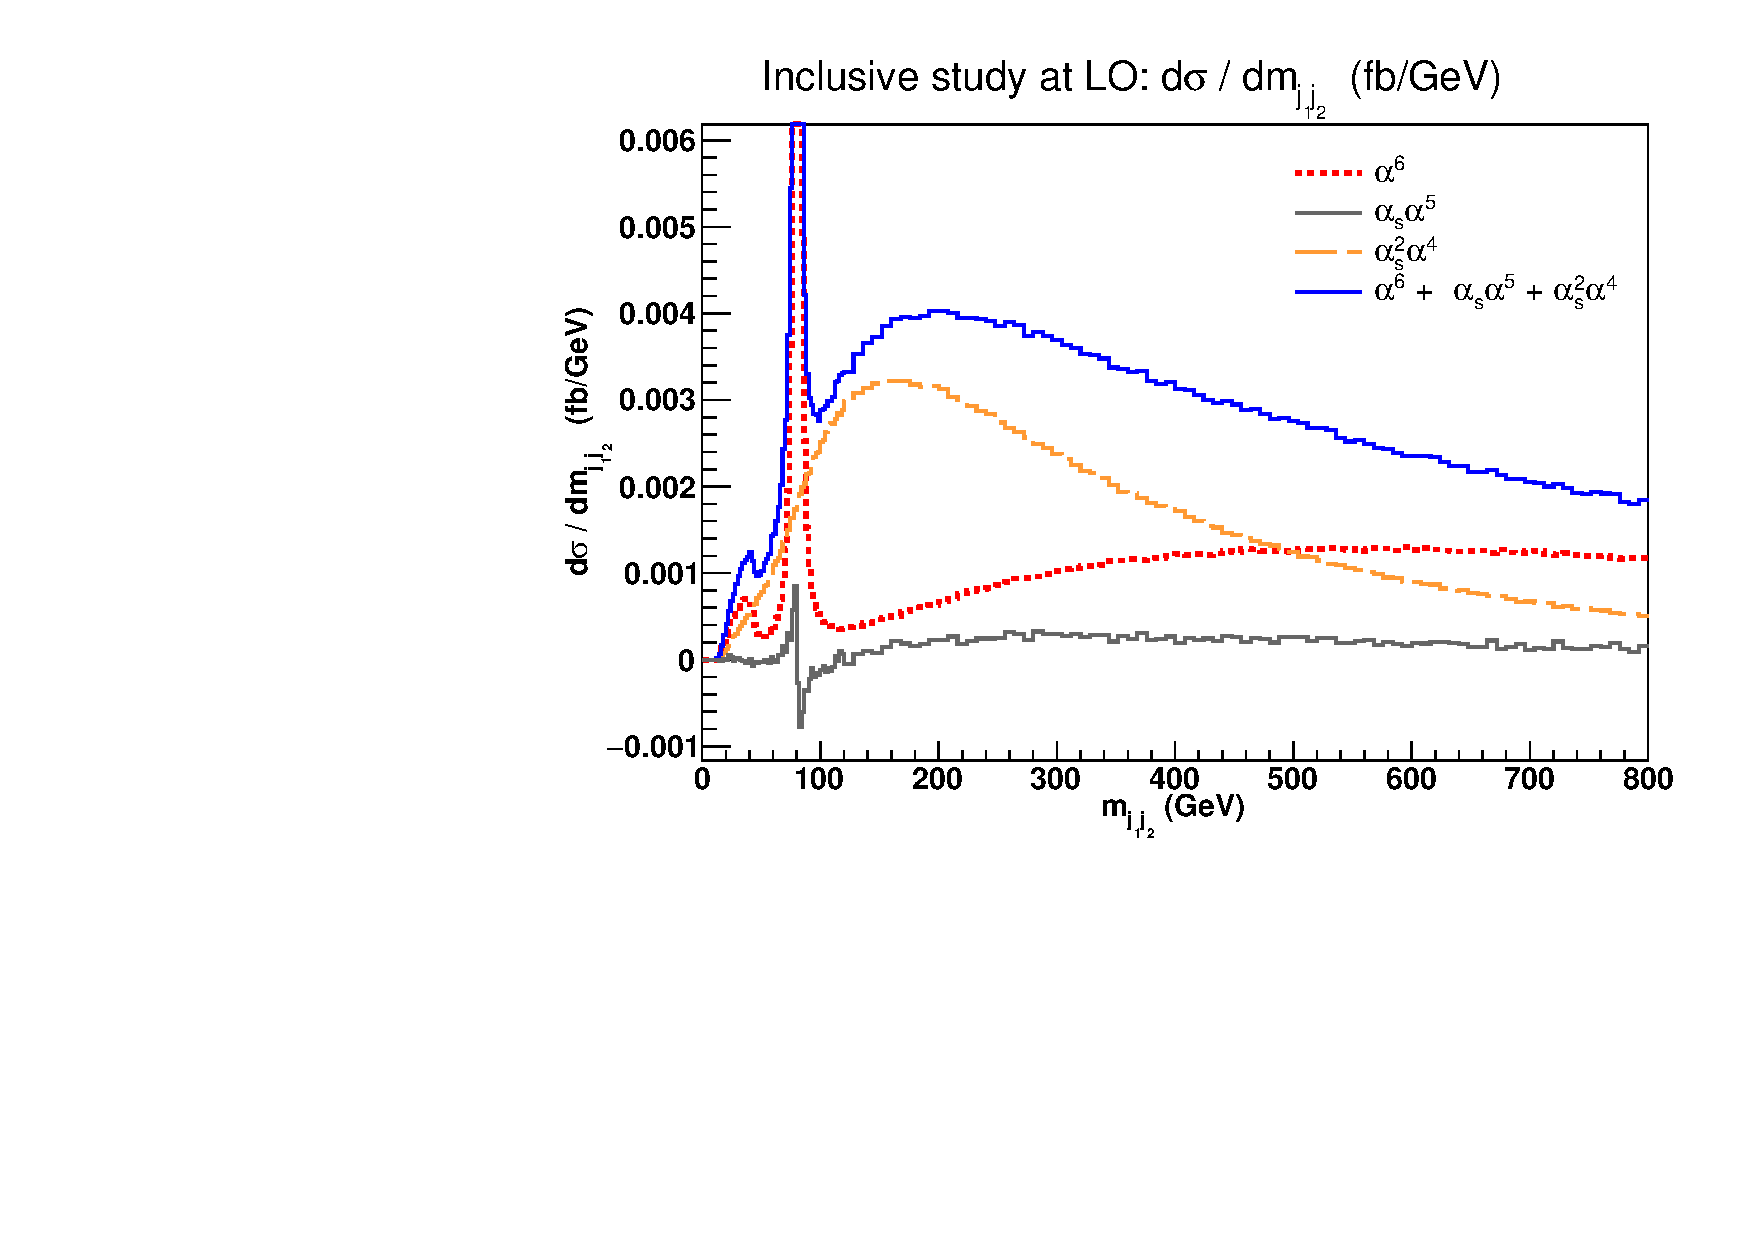
\includegraphics[scale=0.395]{figures/scanfigures/mjj_full.pdf}
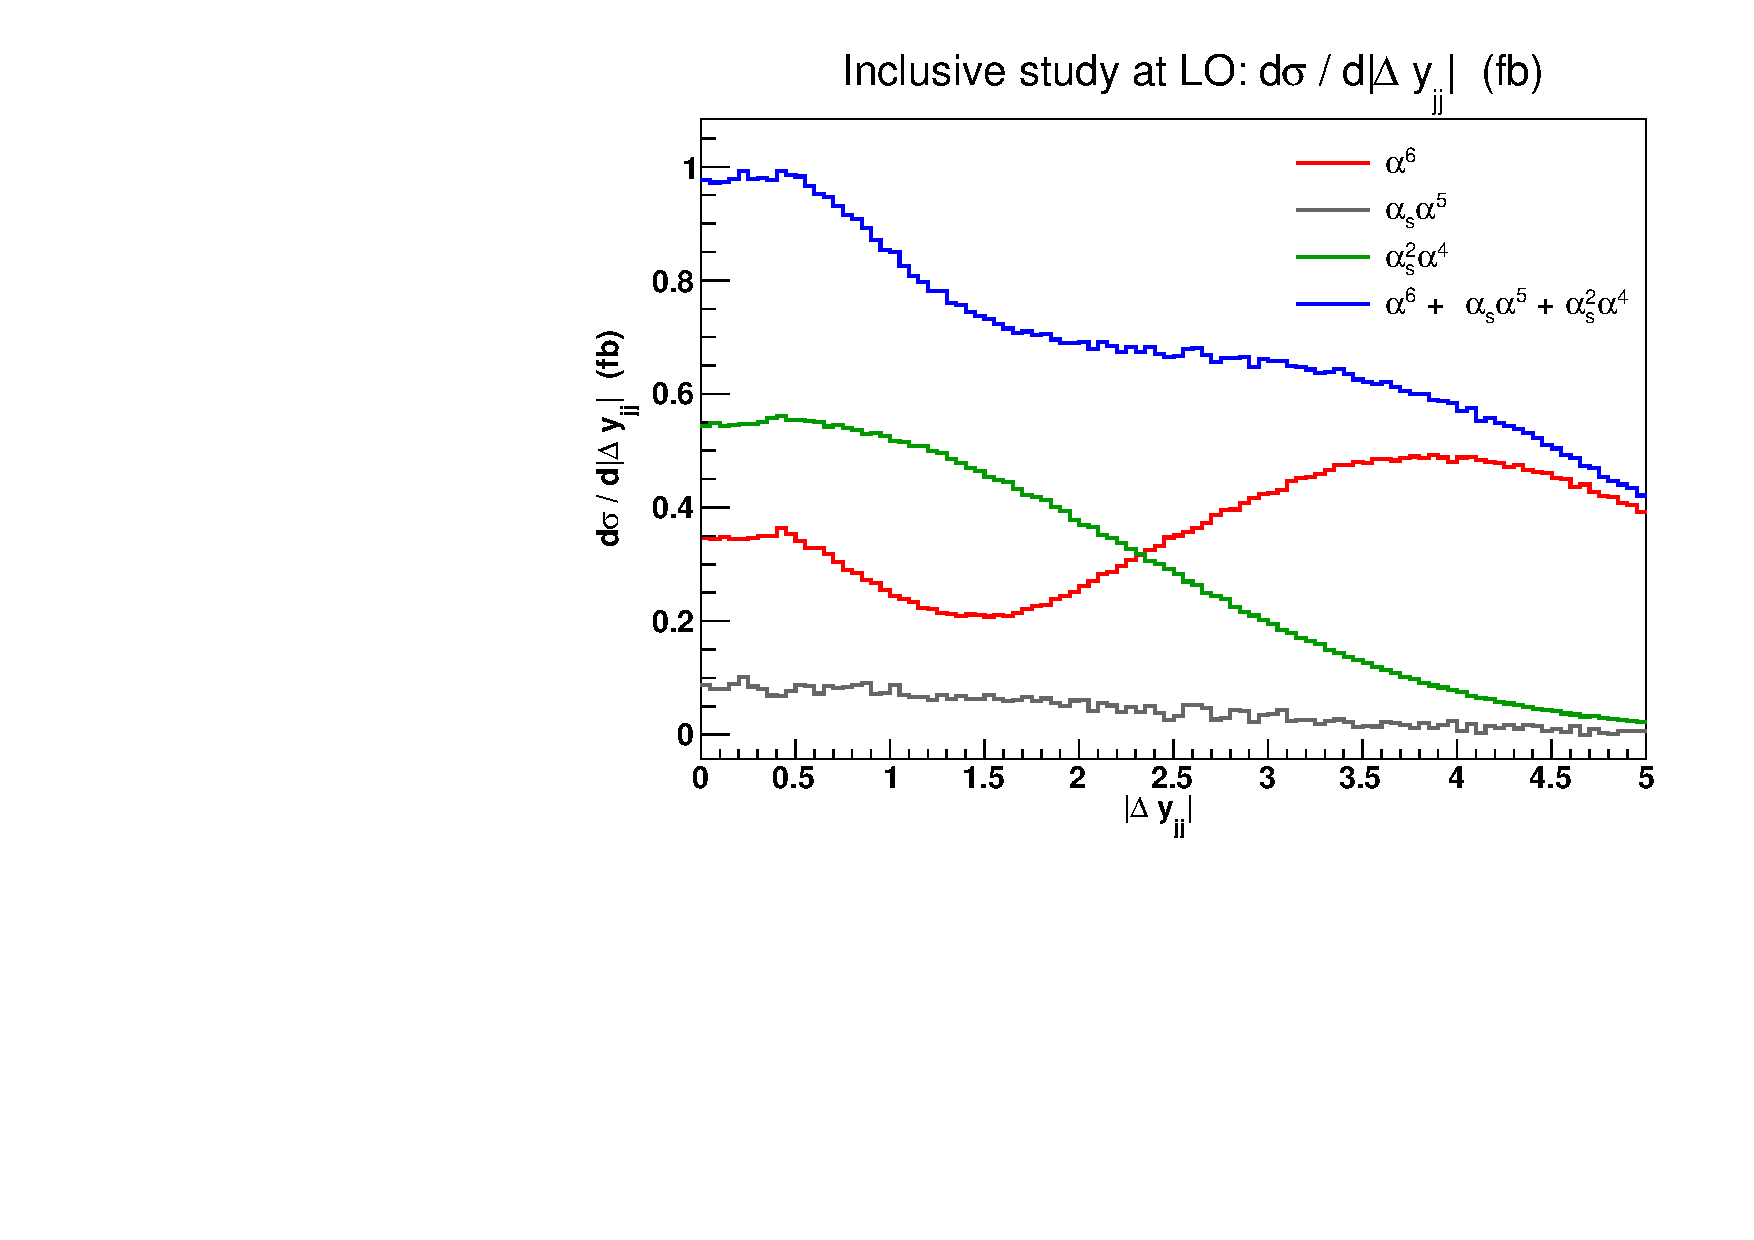
\includegraphics[scale=0.395]{figures/scanfigures/dyjj_full.pdf}
\caption{Differential distribution in the jet--jet invariant mass $M_{jj}$ (left) and the positive difference of the jet rapidities $|\Delta y_{jj}|$ (right) at LO. EW contribution in red, QCD in green, interference in gray and sum in blue. No cuts on $M_{jj}$ and $|\Delta y_{jj}|$ are applied. Results of full LO matrix element simulation.}
\label{fig:mjjdyjj_1d}
\end{figure*}
Concerning the QCD contribution, it is worth noticing that for quantum number conservation external gluons cannot contribute at LO, thus the $\mathcal{O}(\alphas^2\alpha^4)$ diagrams only involve $t/u$--channel virtual gluons: this results in a small QCD background, although the VBF topological cuts are not imposed. The interference between EW and QCD contributions is small, due to color suppression, but not negligible ($t/u$ interference with identical fermions). The LO cross--section for the three perturbative orders are shown in table~\ref{tab:LOscanXsec}.
\begin{table}[h!]
    \centering
    \begin{tabular}{c|c|c|c}
        Code  &  $\sigma[\rm{fb}] (\mathcal{O}(\alpha^6))$ & $\sigma[\rm{fb}] (\mathcal{O}(\alphas^2\alpha^4))$ & $\sigma[\rm{fb}] (\mathcal{O}(\alphas\alpha^5))$ \\
        \hline
        \hline
        {\sc Phantom}  &  $ 2.292 \pm 0.002 $ & $ 1.477 \pm 0.001 $ & $ 0.223 \pm 0.003 $ \\
        {\sc Xxx}&  $ \pm $ & $ \pm $ & $ \pm $
    \end{tabular}
    \caption{\label{tab:LOscanXsec} Cross sections at LO accuracy for the ${\rm p}{\rm p}\to\mu^+\nu_\mu{\rm e}^+\nu_{\rm e}{\rm j}{\rm j}$ process: these results concern the setup described in section~\ref{subsec:inputpar}, apart from the $M_{jj}$ and $|\Delta y_{jj}|$ cuts which have been dropped.}
\end{table}
The EW, QCD and interference amount respectively to 57\%, 37\% and 6\% of the total inclusive cross section. In the presence of typical VBS cuts, the EW contribution is strongly enhanced, as shown in section~\ref{subsec:LOfiducial}.\\
The EW contribution to the $M_{jj}$ distribution (red curve in Fig.~\ref{fig:mjjdyjj_1d}) shows a huge peak around the $W$ mass: this is due to the possibility for the two jets to be decay products of a $W^-$ boson. Note that this effect doesn't arise in calculations which employ VBS approximation (see VBS approx. description in section [ref.]).
One can also see this in three different plots in the plan $\left(m_{\Pj\Pj}, \Delta y_{\Pj\Pj}\right)$.
\begin{figure}[ht]
\centering
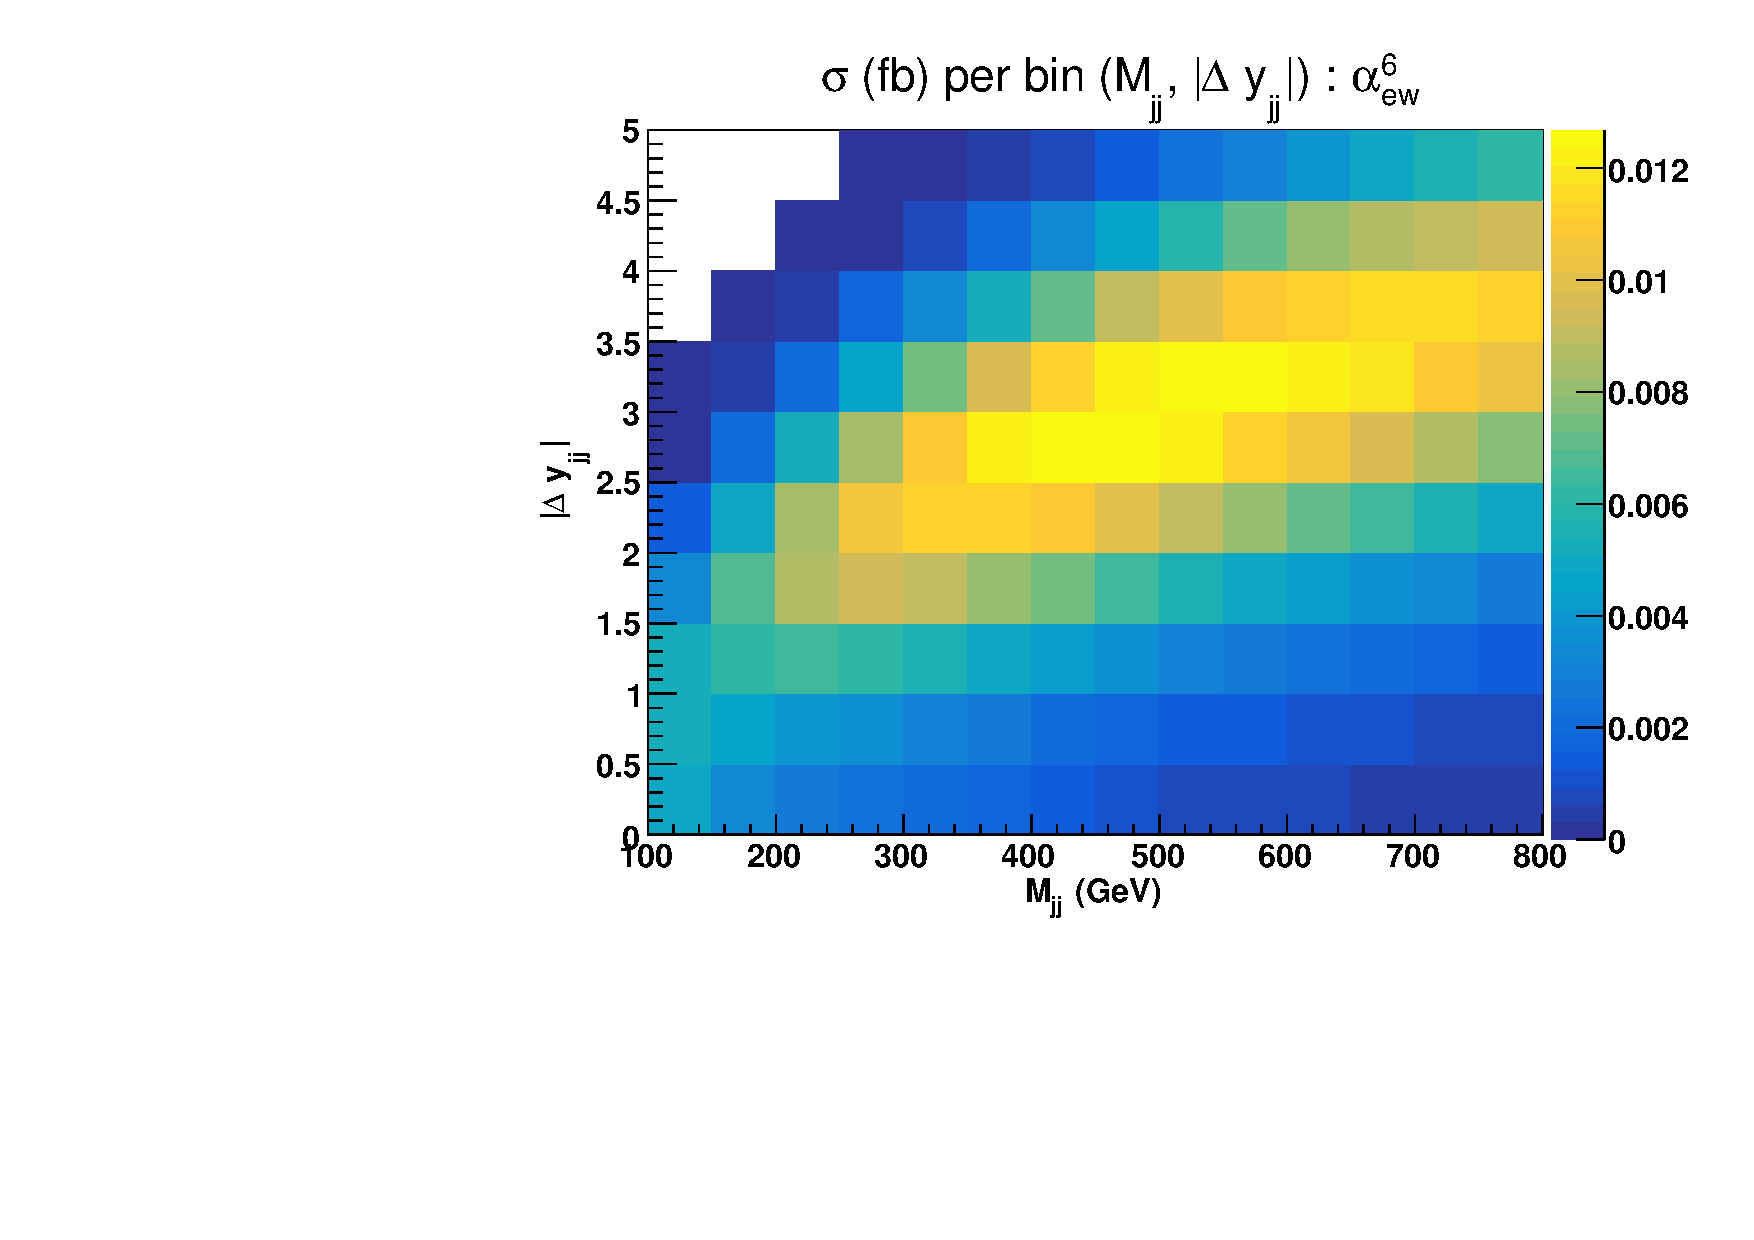
\includegraphics[scale=0.395]{figures/scanfigures/scan_ew6.pdf}
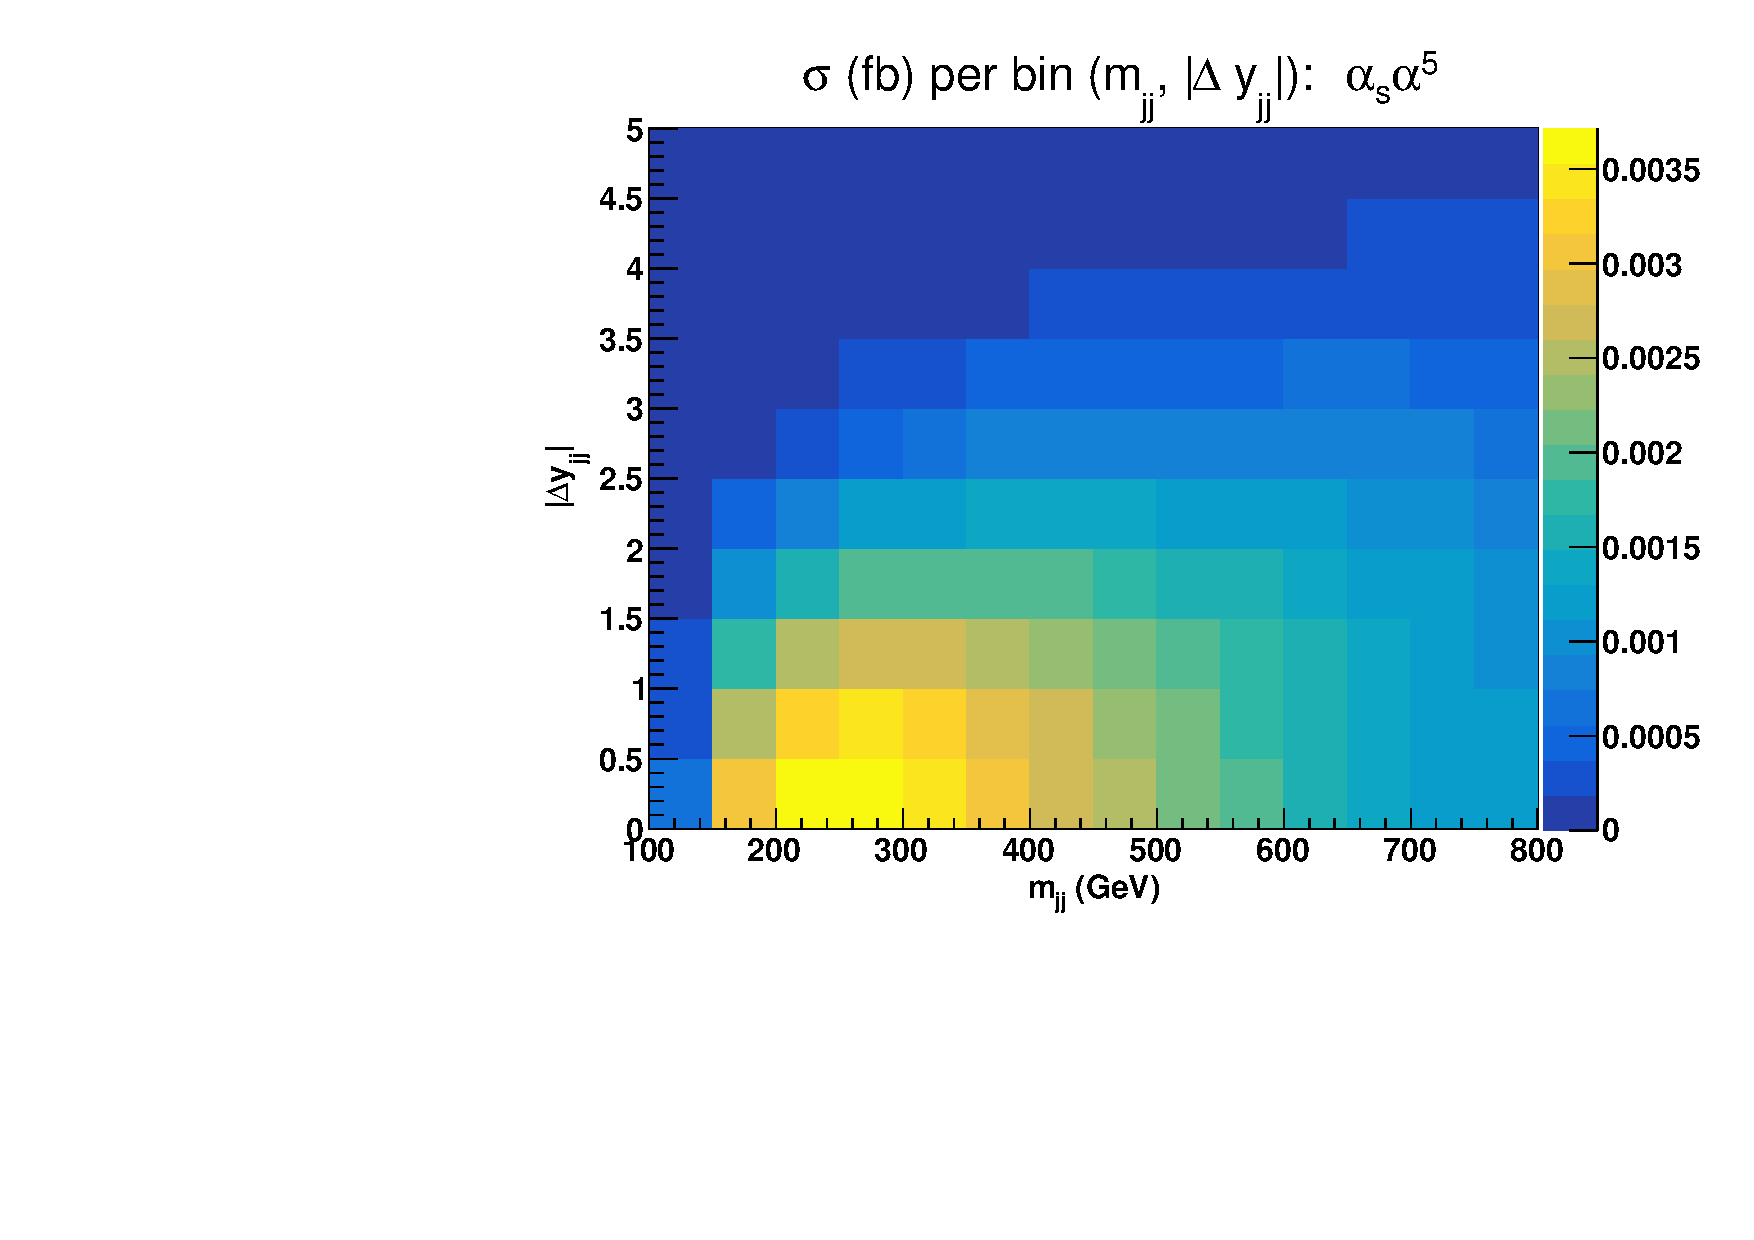
\includegraphics[scale=0.395]{figures/scanfigures/scan_ew5qcd1.pdf}
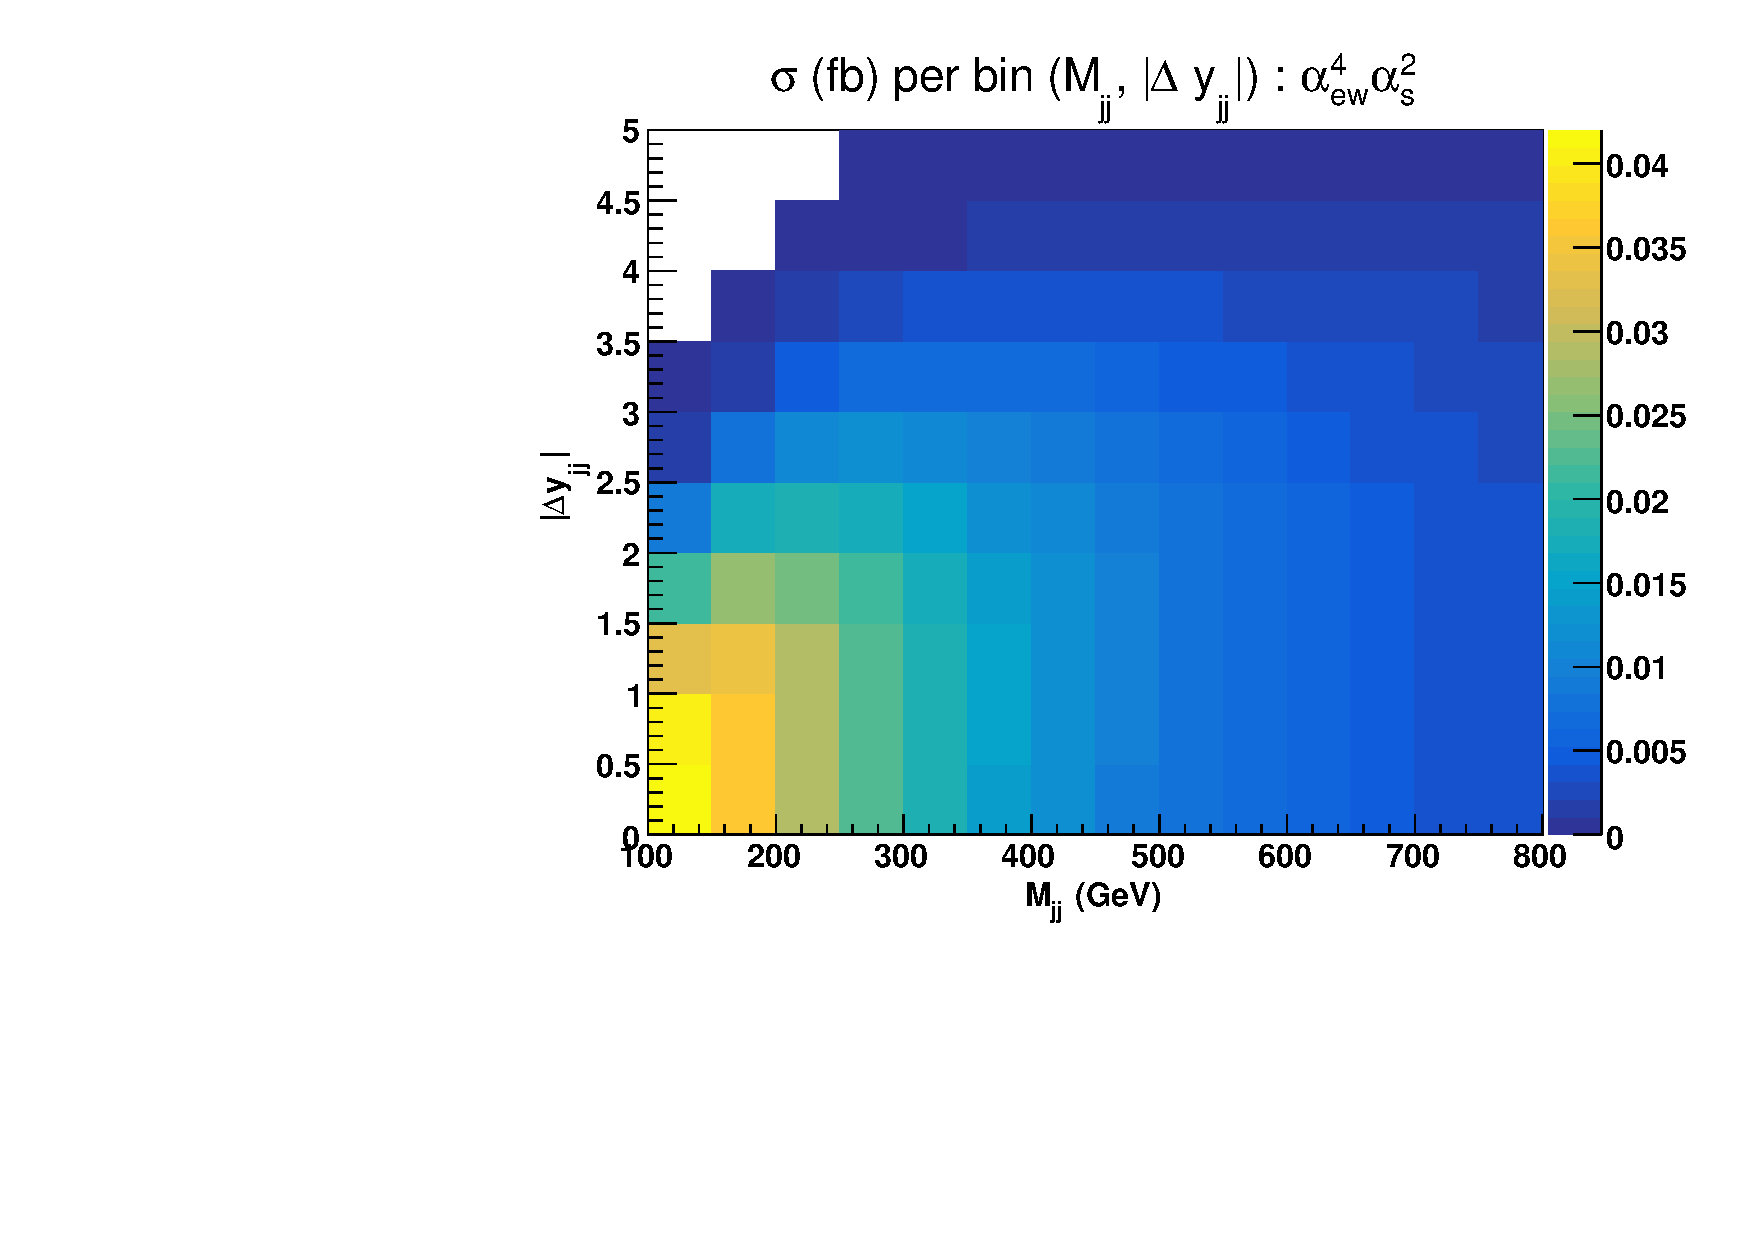
\includegraphics[scale=0.395]{figures/scanfigures/scan_ew4qcd2.pdf}
\caption{Cross sections (fb) per bin in the plan $\left(m_{\Pj\Pj}, \Delta y_{\Pj\Pj}\right)$ for the three LO contributions of orders $\mathcal{O}(\alpha^6)$ (top left), $\mathcal{O}(\alpha^5\alphas)$ (top right), and $\mathcal{O}(\alpha^4 \alphas^2)$ (bottom).}
\label{fig:mjjdyjj_2d_LO}
\end{figure}
